\documentclass{article} % For LaTeX2e
\usepackage{nips15submit_e,times}
\usepackage{hyperref}
\usepackage{graphicx}
\usepackage{amsmath}
\usepackage{amsthm}
\usepackage{graphicx}
\usepackage{lmodern}
\usepackage{titlesec}
\usepackage{longtable}
\usepackage{geometry}
\usepackage{multirow}
\usepackage{listings}
\usepackage{amsfonts}
\usepackage{algorithm}
\usepackage{algpseudocode}
\usepackage{multirow}
\usepackage{array}
\usepackage{url}
\documentstyle[nips14submit_09,times,art10]{article} % For LaTeX 2.09

\author{
Thomas Nedelec \\
MSc Machine Learning\\
\texttt{thomas.nedelec.15@ucl.ac.uk} \\
\And
Michal Daniluk \\
MSc Machine Learning\\
\texttt{michal.daniluk.15@ucl.ac.uk} \\
}
\title{Supervized Learning: Assignment 1}




\newcommand{\fix}{\marginpar{FIX}}
\newcommand{\new}{\marginpar{NEW}}

\nipsfinalcopy % Uncomment for camera-ready version

\begin{document}


\maketitle

\begin{abstract}

\end{abstract}

\section{Exercise 1: Least Square Regression: effect of the training set size}

  \begin{figure}[H]
\center
\begin{tabular}{ccc}
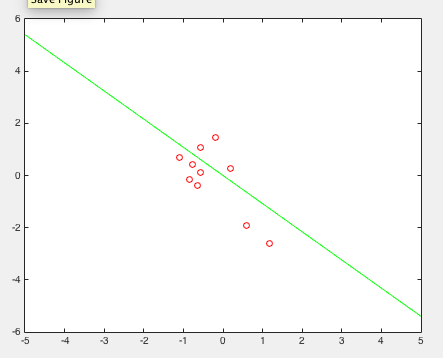
\includegraphics[width=0.3\textwidth]{10points}&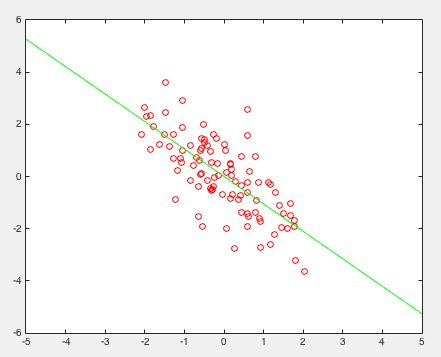
\includegraphics[width=0.3\textwidth]{100points}&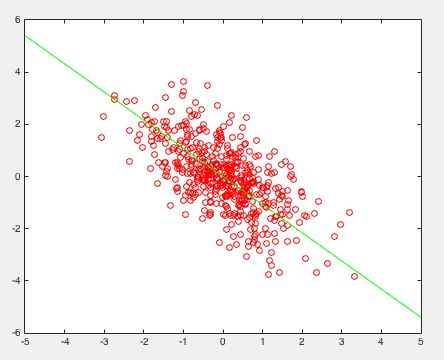
\includegraphics[width=0.3\textwidth]{500points}
\end{tabular}
\caption{ (a) training set of 10 points(b) training set of 100 points (c) the entire data set}
\end{figure}


\begin{figure}[H]
\begin{center}
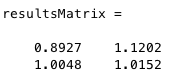
\includegraphics[width=0.4\textwidth]{resultsMatrix}
\end{center}
\caption{Average error on the training set (first row: 10 training points, second row: 100 training points}
\end{figure}

We can observe that increasing the size of training set lets to decrease the average mean error on the test set.

\section{Exercise 2: Least Square Regression: effect of dimensionality}

\begin{figure}[H]
\begin{center}
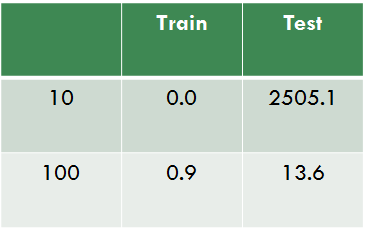
\includegraphics[width=0.4\textwidth]{resultsMatrix2}
\end{center}
\caption{Average error on the training set (first row: 10 training points, second row: 100 training points}
\end{figure}

Interpretation: 

\section{Ridge regression}

The regularization is a way to reduce the freedom of the classifier in order to improve the generalization and reach a better test set average error. 
\\ To implement ridge regression, we would like to minimize according to \textit{w} the cost function, 
\begin{equation}
\gamma w^{T}w + \frac{1}{l} \sum_{i=1}^{l}(x_{i}^{T}w - y_{i})^{2}.
\end{equation}
Using the notation $X=(x_{1}, x_{2},...,x_{l})^{T}$, a matrix containing the training sample vectors as its rows, we can rewrite the cost function as: 
\begin{equation}
\gamma w^{T} w + \frac{1}{l} Tr((Xw - Y)^{T}(Xw - Y))
\end{equation}
Taking derivative according to w, we reach: 
\begin{equation}
2\gamma w + 2 \frac{1}{l} (X^{T}Xw - 2Y^{T}X)=0
\end{equation}
To reach the conditions for optimality, we set the previous equation to zero and we reach: 
\begin{equation}
w=(\gamma l Id +X^{T}X)^{-1}Y^{T}X
\end{equation}
because if $\gamma*l \ne 0$ $(\gamma l Id +X^{T}X)$ is non-singular.
\\\gamma l Id +X^{T}X is symetric.
\\ We consider $u \in \mathbb{R}^{d}$:
\begin{align*}
\langle (\gamma l Id +X^{T}X)u,u \rangle &= \langle \gamma l u,u \rangle + \langle X^{T}X,u \rangle
\\  &= \gamma l \langle  u,u \rangle + \langle X u, X u \rangle
\\ &= \gamma l ||u||^{2} + ||Xu||^{2} > 0 \textit{ for u $\ne$ 0}
\end{align*}
Thus $\gamma l Id +X^{T}X$ is definite positve. 

\section{Effect of the regularisation parameter}

  \begin{figure}[H]
\center
\begin{tabular}{cc}
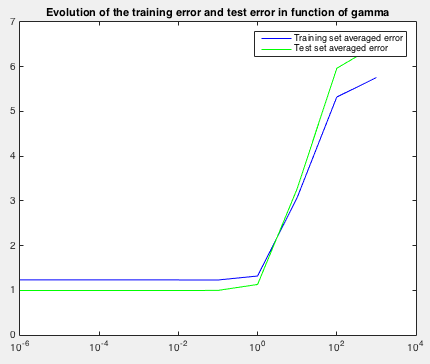
\includegraphics[width=0.5\textwidth]{error4}&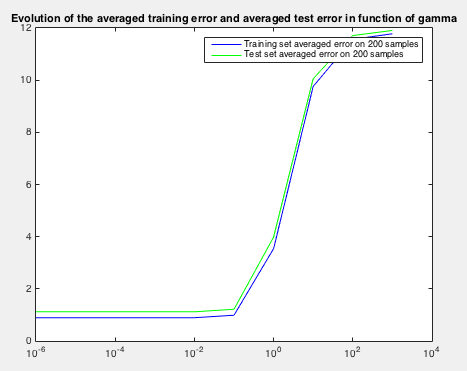
\includegraphics[width=0.5\textwidth]{averagederror4}
\end{tabular}
\caption{ (a) evolution of the training error and test errror for one run (b) evolution of the training error and test error averaged on 200 runs}
\end{figure}

First, the graph shows that if gamma is too high, the training error and test error increase dramatically. It is intuitive because when gamma is high the algorithm is far more likely to minimize $||w||$  rather than the training error.


\\We have an optimal point corresponding to inflection point of the curve in order to select $\gamma$. Nevertheless, the training set error is not a sufficiently good guidance to select the regularization parameter because the charts are quite different. 

\\However, when we average the training error on 200 runs, we can observe that now the test error and the training error are now almost identical.

\\A way to select the optimal $\gamma$ would be to plot the error on the training set averaged on a certain number of runs of the algorithm and select the optimal $\gamma$ on this curve. 


\section{Tuning the regularization parameter using a validation set}



\end{document}
